\section{Fixed-rank benchmark: complete results}
\label{sec:S_legacy}

\subsection{Experiment inventory}

\begin{itemize}
\item \textbf{V1 (extension verification):} fourth-order QR pivots and $\ell_1$ reconstruction are compared with the public TBMD library; the untruncated TBMD--POD-E identity is checked numerically (RQs 1--2).
\item \textbf{E0 (lineage):} re-execution of the archived notebook configuration (Supplementary Section~S2).
\item \textbf{E1 (representation):} full-observation least-squares projection of held-out snapshots onto POD and TBMD for $r\in\{2,\allowbreak 5,\allowbreak 10,\allowbreak 16,\allowbreak 20,\allowbreak 30,\allowbreak 50\}$ and the training-selected depth, and onto TBMD with $R_1\in\{12,\allowbreak 24,\allowbreak 48,\allowbreak 96,\allowbreak 139\}$, $R_2=\min(R_1,48)$, at the selected depth (RQ2).
\item \textbf{E2 (main benchmark):} bases \{POD, POD-E, TBMD\} $\times$ placements \{QR/DG on the same basis, configured order, 20 random orders\} $\times$ estimators \{LS, $\ell_1$\}, plus prior and prior + IDW; 12 grid-wide budgets of 2--300 channels and 10 well budgets of 1--30 wells, with joint (pressure and $S_o$) or pressure-only well sensors; both protocols, all ten folds (RQs 1, 3, 4).
\item \textbf{E3 (noise):} P2, DG-selected wells ($N=10,30$), grid-wide QR ($N=30$) and configured order; five Gaussian-noise levels, ten draws per level (RQ5; Supplementary Section~S3).
\item \textbf{E4 ($\ell_1$ weight):} P2, $\varepsilon\in\{10^{-4},10^{-3},10^{-2},10^{-1}\}$ for QR ($N=10,30,100$) and DG wells ($N=5,10,30$) (RQ5).
\item \textbf{E5 (stability and interpretation):} Jaccard similarity of QR selections and Kendall rank correlation of DG well orders across the ten P2 bases; comparison of selected cells with the training temporal standard deviation and the distance to existing wells (RQ5).
\item \textbf{E6 (cost):} single-thread wall time of offline (SVD, Tucker, QR, DG) and online (per-snapshot LS and $\ell_1$) steps, median of repeated runs (RQ5).
\item \textbf{E8 (property coupling):} joint fourth-order versus independent third-order TBMD, identical folds and measurements at 10 or 30 configured wells, matched total or per-property coefficient counts, LS and $\ell_1$ (RQ2; Supplementary Section~S4).
\item \textbf{E9 (third versus fourth order):} a frozen nested comparison of independent third-order TBMD with five fourth-order coupling architectures under equal-total and equal-per-property capacities; full observation, 5--30 configured wells and 30--300 common grid channels; property-wise reconstruction error, mask-aware SSIM and RMSE; all ten P2 outer folds (RQ6; the main manuscript). E9 supersedes E8 for the dimensionality question but retains E8 as provenance for the original rigid formulation.
\item \textbf{O1--O5 (nested optimization):} train-only representation search; recovery tuning; placement tuning; bounded joint refinement; one outer evaluation; prespecified placement audit; and independent frozen refitting. The registry contains \OptValidationRecords{} sparse validation records and \OptOuterRecords{} outer records (RQs 1--5; the main manuscript).
\end{itemize}


\subsection{References without measurements and the choice of protocol}
\label{sec:res_protocol}
The field-mean pressure of all scenarios falls during early production, recovers and then varies slowly (Fig.~\ref{fig:data}a). The scenarios differ by a persistent pressure deviation whose cross-scenario standard deviation, averaged over cells, peaks at \CrossSdMax{} $u_p$ and is \CrossSdEnd{} $u_p$ at the last snapshot (Fig.~\ref{fig:data}b). Over the P1 hold-out window, persistence of the last training snapshot has a pressure RMSE that grows from \PersistFirst{} $u_p$ at the first held-out snapshot to \PersistLast{} $u_p$ at the last one. Averaged over the window and the ten scenarios, persistence reaches $\mathrm{RMSE}_p=\POnePriorGridTenP\pm\POnePriorGridTenPsd\,u_p$ and $\mathrm{RMSE}_{S_o}=\POnePriorGridTenS\times10^{-3}$ (Table~\ref{tab:S_P1}). In P2, the ensemble mean of the other scenarios reaches $\PTwoPriorGridTenP\pm\PTwoPriorGridTenPsd\,u_p$ and $\PTwoPriorGridTenS\times10^{-3}$. Saturation differences between scenarios are therefore very small. Because persistence is already accurate in P1, the main comparisons use P2.

\begin{figure}[tbp]
\centering
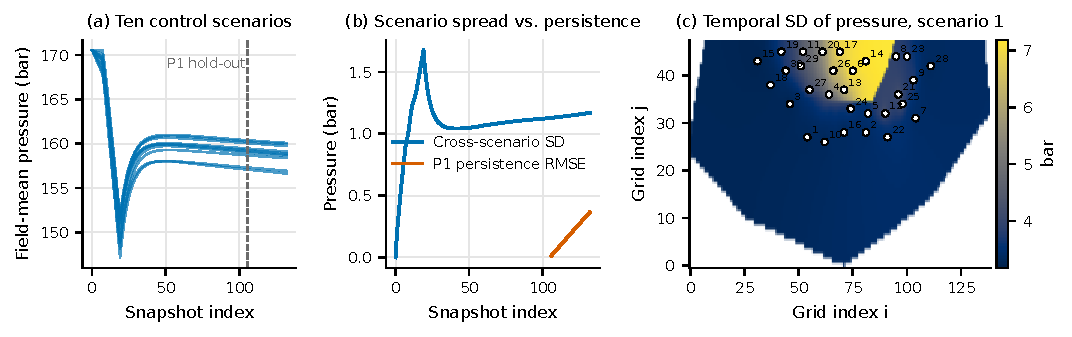
\includegraphics[width=\textwidth]{../../../../studies/brugge_sparse_sensing/figures/fig2_data_context.pdf}
\caption{Brugge control ensemble used in this study. (a) Field-mean pressure (supplied export unit $u_p$) of the ten control scenarios against snapshot index; the dashed line marks the start of the P1 hold-out window. (b) Cross-scenario standard deviation of pressure, averaged over active cells, and pressure RMSE of persistence of the last training snapshot over the P1 window (mean over scenarios). (c) Temporal standard deviation of pressure in scenario~1 on the $139\times48$ grid (inactive cells blank), with the 30 existing wells labelled by their configured order.}
\label{fig:data}
\end{figure}


\subsection{Representation capacity of the bases (RQ1)}
\label{sec:res_representation}
The energy criterion selects $r=\RankPTwoMin$ in every P2 fold and $r\in\{\RankPOneMin,\RankPOneMax\}$ in P1. With all active channels observed, the POD and POD-E bases (which share a subspace) reproduce held-out P2 states with $\mathrm{RMSE}_p=\EOnePTwoPodOracle\,u_p$, while TBMD with $(R_1,R_2,R_3)=(48,48,2)$ reaches only \EOnePTwoTbmdOracle{} $u_p$ at the same depth (Fig.~\ref{fig:representation}a,b). This TBMD floor is about \EOnePTwoFloorRatio{} times the POD error and does not decrease with depth, because it is set by the spatial truncation (Fig.~\ref{fig:representation}c). The TBMD error decreases monotonically with $R_1$ and coincides with POD at $R_1=139$, as Proposition~1 of the main manuscript predicts; numerically, the relative difference of the singular values and the subspace distance are both below \PropSvDiff{}. In P1 the TBMD floor (\EOnePOneTbmdOracle{} $u_p$) already exceeds the error of persistence (\POnePriorGridTenP{} $u_p$); consistently, no TBMD configuration in P1 improved on persistence (best mean error \POneTbmdBest{} $u_p$; Supplementary Table~S3).

\begin{figure}[tbp]
\centering
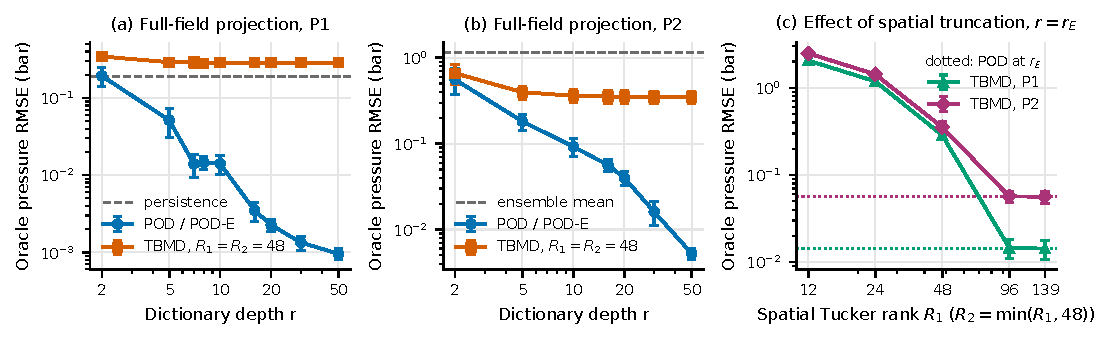
\includegraphics[width=\textwidth]{../../../../studies/brugge_sparse_sensing/figures/fig3_representation.pdf}
\caption{Representation capacity with all active channels observed (least-squares projection of held-out snapshots). (a, b) Pressure RMSE against dictionary depth $r$ for POD/POD-E (identical subspace) and TBMD with spatial ranks $(48,48,2)$ in P1 and P2; dashed line: no-measurement reference. (c) TBMD pressure RMSE against the spatial Tucker rank $R_1$ ($R_2=\min(R_1,48)$, $R_3=2$) at the training-selected depth; dotted lines: POD at the same depth. Markers: mean over ten folds; bars: one standard deviation.}
\label{fig:representation}
\end{figure}


\subsection{Grid-wide sensing (RQs 3 and 5)}
\label{sec:res_grid}
Figure~\ref{fig:budget}a and Table~\ref{tab:main} show three regimes for grid-wide channels in P2.
\emph{Below the depth ($N<r$)} the orthonormal POD basis fails: with $N=10$ QR-selected channels, POD gives $\PTwoPodLsGridTenP\,u_p$ with LS and $\PTwoPodLoneGridTenP\,u_p$ with $\ell_1$. The energy-weighted bases remain below the prior. POD-E with LS gives $(\PTwoPodeLsGridTenP\pm\PTwoPodeLsGridTenPsd)\,u_p$ (better than POD LS in \WPTwoPodELsVsPodLsGridTenWins{} of 10 folds, $p=\WPTwoPodELsVsPodLsGridTen$), and TBMD with $\ell_1$ gives $(\PTwoTbmdLoneGridTenP\pm\PTwoTbmdLoneGridTenPsd)\,u_p$.
\emph{At and above the depth} POD and POD-E agree for the same measurement rows when the sampled basis has full column rank; their separately optimised placements need not coincide. With $N=30$ channels the error is $(\PTwoPodeLsGridThirtyP\pm\PTwoPodeLsGridThirtyPsd)\,u_p$, a factor of about \PTwoGainPriorGridThirty{} below the prior. POD-E LS is lower than prior + IDW ($\PTwoIdwGridThirtyP\,u_p$) and than the original TBMD configuration ($\PTwoTbmdLoneGridThirtyP\,u_p$) in \WPTwoQrPodELsVsIdwGridThirtyWins{} and \WPTwoQrPodELsVsQrTbmdLGridThirtyWins{} of 10 folds, respectively ($p=\WPTwoQrPodELsVsIdwGridThirty$ in both cases). With $N=100$ channels POD-E LS reaches $\PTwoPodeLsGridHundredP\,u_p$, whereas TBMD saturates at $\PTwoTbmdLoneGridHundredP\,u_p$, close to its representation floor.
\emph{Placement} matters. At $N=30$, QR-selected channels give a lower error than the median of 20 random selections in \WPTwoQrPodELsVsRandomMedianGridThirtyWins{} of 10 folds ($p=\WPTwoQrPodELsVsRandomMedianGridThirty$; random median $\PTwoRandLsGridThirtyP\,u_p$). At $N=10$ they are better in \WPTwoQrPodELsVsRandomMedianGridTenWins{} folds ($p=\WPTwoQrPodELsVsRandomMedianGridTen$).
Saturation errors change little: POD-E LS gives $\PTwoPodeLsGridHundredS\times10^{-3}$ at $N=100$ against $\PTwoPriorGridTenS\times10^{-3}$ for the prior, and prior + IDW increases the saturation error (Supplementary Table~S4).

\begin{figure}[tbp]
\centering
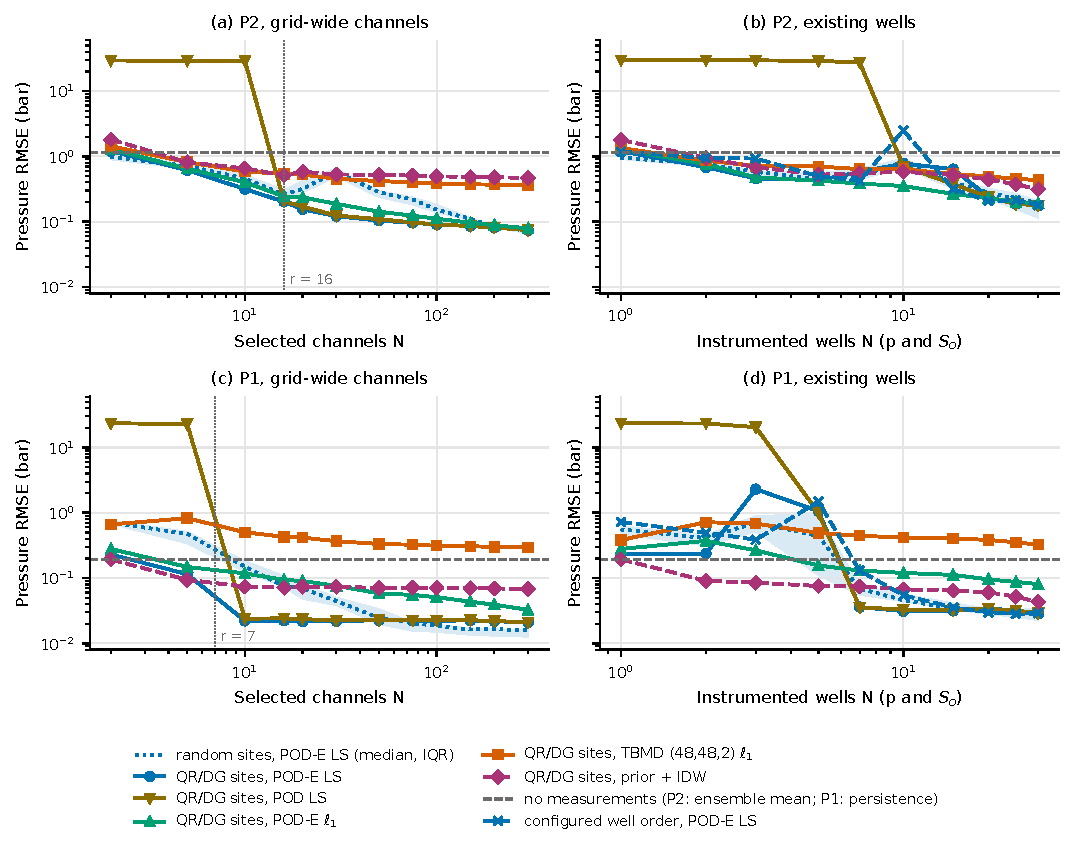
\includegraphics[width=\textwidth]{../../../../studies/brugge_sparse_sensing/figures/fig4_budget_curves.pdf}
\caption{Pressure RMSE (supplied export unit $u_p$; mean over ten folds) against the measurement budget. (a) P2, grid-wide channels; (b) P2, existing wells measuring pressure and $S_o$; (c, d) the same for P1. QR: pivoted-QR/determinant-greedy channels; DG: determinant-greedy well order; both computed on the basis named in the legend. The shaded band and dotted line show the interquartile range and median over folds of the per-fold median of 20 random placements (POD-E, LS). Dashed grey: no-measurement reference; vertical dotted line: dictionary depth $r$. Axes are logarithmic; standard deviations are given in Table~\ref{tab:main}.}
\label{fig:budget}
\end{figure}

\begin{table}[tbp]
\centering
\scriptsize
\setlength{\tabcolsep}{2.5pt}
\caption{Pressure RMSE (bar) in protocol P2, mean\,$\pm$\,standard deviation over the ten held-out control scenarios. Placement is QR (grid) or DG (wells) on the basis of the same row unless stated; $r=16$ in every fold. The prior row uses no measurements and is repeated across columns. Random: per-fold median over 20 placements.}
\label{tab:main}
\begin{tabular}{@{}lcccccc@{}}
\toprule
 & \multicolumn{3}{c}{Grid-wide channels} & \multicolumn{2}{c}{Wells ($p$, $S_o$)} & Wells ($p$) \\
\cmidrule(lr){2-4}\cmidrule(lr){5-6}\cmidrule(l){7-7}
Method & $N=10$ & $N=30$ & $N=100$ & $N=10$ & $N=30$ & $N=30$ \\
\midrule
No measurements (prior) & 1.15\,$\pm$\,0.56 & 1.15\,$\pm$\,0.56 & 1.15\,$\pm$\,0.56 & 1.15\,$\pm$\,0.56 & 1.15\,$\pm$\,0.56 & 1.15\,$\pm$\,0.56 \\
Prior + IDW (POD-E sites) & 0.65\,$\pm$\,0.35 & 0.53\,$\pm$\,0.27 & 0.50\,$\pm$\,0.26 & 0.58\,$\pm$\,0.24 & 0.31\,$\pm$\,0.16 & 0.31\,$\pm$\,0.16 \\
POD, LS & 29\,$\pm$\,1 & 0.12\,$\pm$\,0.04 & 0.09\,$\pm$\,0.02 & 0.70\,$\pm$\,0.30 & 0.18\,$\pm$\,0.09 & 0.23\,$\pm$\,0.09 \\
POD, $\ell_1$ & 31\,$\pm$\,1 & 2.01\,$\pm$\,0.27 & 0.78\,$\pm$\,0.13 & 11\,$\pm$\,3 & 1.04\,$\pm$\,0.24 & 5.04\,$\pm$\,0.70 \\
POD-E, LS & 0.32\,$\pm$\,0.18 & 0.12\,$\pm$\,0.04 & 0.09\,$\pm$\,0.02 & 0.78\,$\pm$\,0.45 & 0.18\,$\pm$\,0.09 & 0.23\,$\pm$\,0.09 \\
POD-E, $\ell_1$ & 0.40\,$\pm$\,0.18 & 0.19\,$\pm$\,0.03 & 0.11\,$\pm$\,0.02 & 0.35\,$\pm$\,0.10 & 0.19\,$\pm$\,0.03 & 0.21\,$\pm$\,0.08 \\
TBMD $(48,48,2)$, LS & 0.54\,$\pm$\,0.08 & 0.42\,$\pm$\,0.06 & 0.38\,$\pm$\,0.06 & 1.27\,$\pm$\,0.38 & 0.43\,$\pm$\,0.05 & 0.48\,$\pm$\,0.05 \\
TBMD $(48,48,2)$, $\ell_1$ & 0.59\,$\pm$\,0.12 & 0.45\,$\pm$\,0.07 & 0.38\,$\pm$\,0.06 & 0.64\,$\pm$\,0.13 & 0.43\,$\pm$\,0.06 & 0.43\,$\pm$\,0.06 \\
Random sites, POD-E, LS & 0.45\,$\pm$\,0.12 & 0.59\,$\pm$\,0.13 & 0.16\,$\pm$\,0.03 & 0.84\,$\pm$\,0.27 & 0.18\,$\pm$\,0.09 & 0.23\,$\pm$\,0.09 \\
Configured wells, POD-E, LS & -- & -- & -- & 2.50\,$\pm$\,1.55 & 0.18\,$\pm$\,0.09 & 0.23\,$\pm$\,0.09 \\
Configured wells, TBMD, $\ell_1$ & -- & -- & -- & 0.47\,$\pm$\,0.07 & 0.43\,$\pm$\,0.06 & 0.43\,$\pm$\,0.06 \\
\bottomrule
\end{tabular}
\end{table}


\subsection{Existing wells (RQs 3--4)}
\label{sec:res_wells}
With measurements restricted to the \NWells{} existing wells, each contributing pressure and $S_o$ (Fig.~\ref{fig:budget}b), prior + IDW is a strong reference: with all wells it reaches $(\PTwoIdwWellThirtyP\pm\PTwoIdwWellThirtyPsd)\,u_p$ and is better than the prior in \WPTwoIdwVsPriorWellsJointThirtyWins{} of 10 folds. With all 30 wells, POD-E gives $(\PTwoPodeLsWellThirtyP\pm\PTwoPodeLsWellThirtyPsd)\,u_p$ with LS and $(\PTwoPodeLoneWellThirtyP\pm\PTwoPodeLoneWellThirtyPsd)\,u_p$ with $\ell_1$. The $\ell_1$ estimate is better than prior + IDW in \WPTwoPodELVsIdwWellsJointThirtyWins{} of 10 folds ($p=\WPTwoPodELVsIdwWellsJointThirty$); the LS estimate only in \WPTwoPodELsVsIdwWellsJointThirtyWins{} ($p=\WPTwoPodELsVsIdwWellsJointThirty$). Both are better than the original TBMD configuration ($\PTwoTbmdLoneWellThirtyP\,u_p$) in all folds.

With ten wells (20 channels for $r=\RankPTwoMin$) the least-squares problem is poorly conditioned \cite{peherstorfer2020}: the median condition number of the sensing matrix is \CondDgTen{} for DG-selected wells, \CondRandTen{} for random wells and \CondConfTen{} for the configured order, against \CondDgThirty{} with all 30 wells. POD-E LS gives $(\PTwoPodeLsWellTenP\pm\PTwoPodeLsWellTenPsd)\,u_p$ with DG-selected wells and $(\PTwoConfLsWellTenP\pm\PTwoConfLsWellTenPsd)\,u_p$ with the configured order. DG ordering is better than the configured order in \WPTwoDgVsConfiguredPodELsWellsJointTenWins{} of 10 folds ($p=\WPTwoDgVsConfiguredPodELsWellsJointTen$), but LS is not consistently better than the prior (\WPTwoPodELsVsPriorWellsJointTenWins{} of 10 folds). The $\ell_1$ estimator on POD-E removes this instability: $(\PTwoPodeLoneWellTenP\pm\PTwoPodeLoneWellTenPsd)\,u_p$, better than the prior in \WPTwoPodELVsPriorWellsJointTenWins{}, than prior + IDW in \WPTwoPodELVsIdwWellsJointTenWins{} ($p=\WPTwoPodELVsIdwWellsJointTen$) and than TBMD $\ell_1$ in \WPTwoPodELVsTbmdLWellsJointTenWins{} of 10 folds. With $\ell_1$ the well order matters little: \LoneDgTen{} $u_p$ (DG), \LoneConfTen{} $u_p$ (configured) and \LoneRandTen{} $u_p$ (median of random orders).

Pressure-only gauges at all 30 wells give $\PTwoPodeLsPWellThirtyP\,u_p$ with POD-E LS, close to joint sensing, so the saturation channel adds little to pressure reconstruction. Inferring $S_o$ from pressure through the joint basis, however, increases the saturation error by more than an order of magnitude ($\PTwoPodeLsPWellThirtyS\times10^{-3}$ against $\PTwoPriorGridTenS\times10^{-3}$; Supplementary Table~S4). Joint well measurements reduce the saturation error relative to the prior in \WPTwoPodELsVsPriorSoWellsJointThirtyWins{} of 10 folds ($p=\WPTwoPodELsVsPriorSoWellsJointThirty$), i.e. not consistently.

Figure~\ref{fig:time} resolves the P2 errors in time for ten DG-selected wells. At the first snapshot all scenarios share the initial state, so the prior and prior + IDW are exact, whereas POD-E $\ell_1$ has a median error of \TimeLoneFirst{} $u_p$. From snapshot \TimeCrossover{} onwards the POD-E $\ell_1$ error stays below the prior error. Its median error is \TimeLoneEarly{} $u_p$ over snapshots 0--30, which include the production transient, and \TimeLoneLate{} $u_p$ afterwards; the prior gives \TimePriorEarly{} and \TimePriorLate{} $u_p$ over the same periods.

\begin{figure}[tbp]
\centering
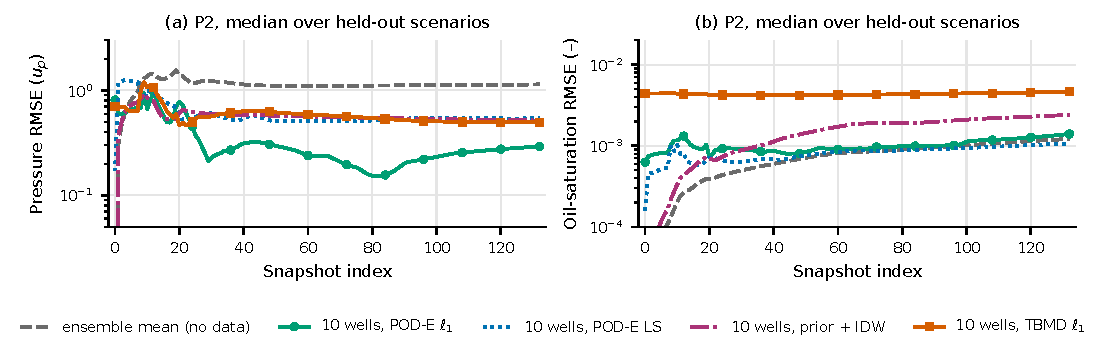
\includegraphics[width=\textwidth]{../../../../studies/brugge_sparse_sensing/figures/fig5_time_resolved.pdf}
\caption{Time-resolved errors in P2 for ten DG-selected wells measuring pressure and $S_o$: median over the ten held-out scenarios of (a) pressure RMSE and (b) oil-saturation RMSE at each snapshot, for the ensemble-mean prior, prior + IDW, POD-E with $\ell_1$ and with least squares, and TBMD $(48,48,2)$ with $\ell_1$.}
\label{fig:time}
\end{figure}


\subsection{Robustness, stability and cost (RQs 3--5)}
\label{sec:res_robust}
\textbf{Noise.} Figure~\ref{fig:noise} shows that least squares with ten wells amplifies measurement noise strongly: POD-E LS rises to \NoiseWellTenPodeLsSigOne{} $u_p$ at $\sigma_p=1\,u_p$, whereas POD-E $\ell_1$ gives \NoiseWellTenPodeLoneSigOne{} $u_p$ and prior + IDW \NoiseWellTenIdwSigOne{} $u_p$. With 30 wells the difference is smaller: \NoiseWellThirtyPodeLsSigOne{} $u_p$ for LS, \NoiseWellThirtyPodeLoneSigOne{} $u_p$ for $\ell_1$ and \NoiseWellThirtyIdwSigOne{} $u_p$ for IDW at $\sigma_p=1\,u_p$. At $\sigma_p=2\,u_p$ the $\ell_1$ and IDW errors are close to the prior error with ten wells (\NoiseWellTenPodeLoneSigTwo{} and \NoiseWellTenIdwSigTwo{} $u_p$) and below it with 30 wells (\NoiseWellThirtyPodeLoneSigTwo{} and \NoiseWellThirtyIdwSigTwo{} $u_p$), whereas least squares exceeds the prior error in both cases (\NoiseWellTenPodeLsSigTwo{} and \NoiseWellThirtyPodeLsSigTwo{} $u_p$).

\textbf{$\ell_1$ weight.} POD-E and TBMD change moderately for $\varepsilon=10^{-4}$--$10^{-2}$ and worsen at $10^{-1}$. Orthogonal POD fails below the depth for every tested weight because its coefficients are large relative to the penalty (Supplementary Fig.~S1). Although $\varepsilon=10^{-3}$ lowers POD-E error in four of six designs, we retain the fixed $10^{-2}$ value because that observation used held-out scenarios; retuning would require a separate validation split.

\textbf{Stability and interpretation.} QR selections for POD-E at $N=50$ overlap between leave-one-out bases with a mean Jaccard index of \StabJacPodeFifty{}, and \StabSharePPodeFifty{}\,\% of the selected channels are pressure channels. On average, the selected cells lie at percentile \StabTstdPodeFifty{} of the training temporal standard deviation of the measured property, and their mean distance to the nearest existing well is \StabDistPodeFifty{} cells, against \StabDistActive{} cells over all active cells; the placement therefore concentrates on dynamically active regions around wells (Fig.~\ref{fig:maps}a). DG rankings of existing wells are consistent across folds (mean Kendall $\tau=\StabTauPode$; Fig.~\ref{fig:maps}b).

\textbf{Cost.} On one CPU thread (P2, $r=16$, \NT{}$\times$9 training snapshots), the POD basis takes \CostPodSvd{} s and the Tucker model \CostTucker{} s. TBMD-based QR placement of $r$ sensors takes \CostQr{} ms and DG ranking of 30 wells \CostBlockDg{} ms. Online POD-E coefficient estimation from 30 wells takes \CostLsWell{}\,\si{\micro\second} with LS and \CostLoneWell{}\,\si{\micro\second} with ADMM per snapshot (fold-amortised, excluding full-state synthesis and inverse scaling; Table~\ref{tab:cost}). The TBMD factors store \TbmdStorage{} numbers against \BasisStorage{} for an explicit basis matrix.

\begin{figure}[tbp]
\centering
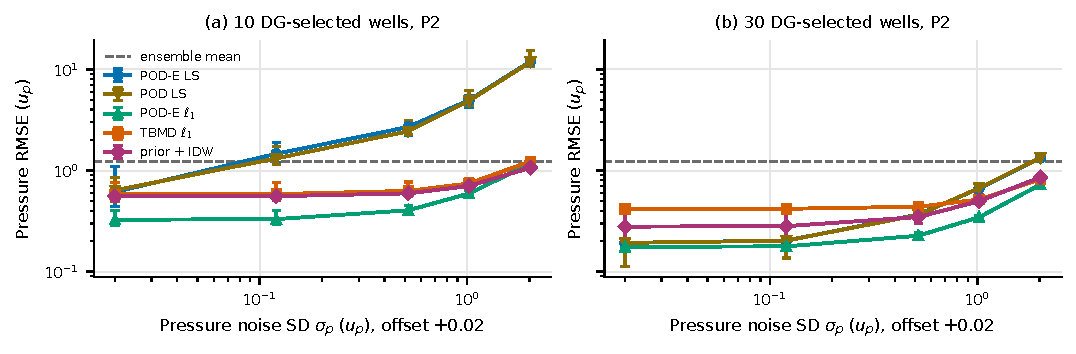
\includegraphics[width=\textwidth]{../../../../studies/brugge_sparse_sensing/figures/fig6_noise.pdf}
\caption{Effect of measurement noise in P2 for (a) 10 and (b) 30 DG-selected wells measuring pressure and $S_o$. Noise standard deviations are $(\sigma_p,\sigma_{S_o})\in\{(0,0),(0.1,0.005),(0.5,0.01),(1,0.02),(2,0.05)\}$ in ($u_p$, dimensionless); the horizontal axis shows $\sigma_p+0.02\,u_p$ so that the noise-free case appears on the logarithmic axis. Markers: median over folds of the per-fold mean over ten noise draws (one evaluation at zero noise); bars: interquartile range over folds; dashed grey: ensemble-mean prior.}
\label{fig:noise}
\end{figure}

\begin{figure}[tbp]
\centering
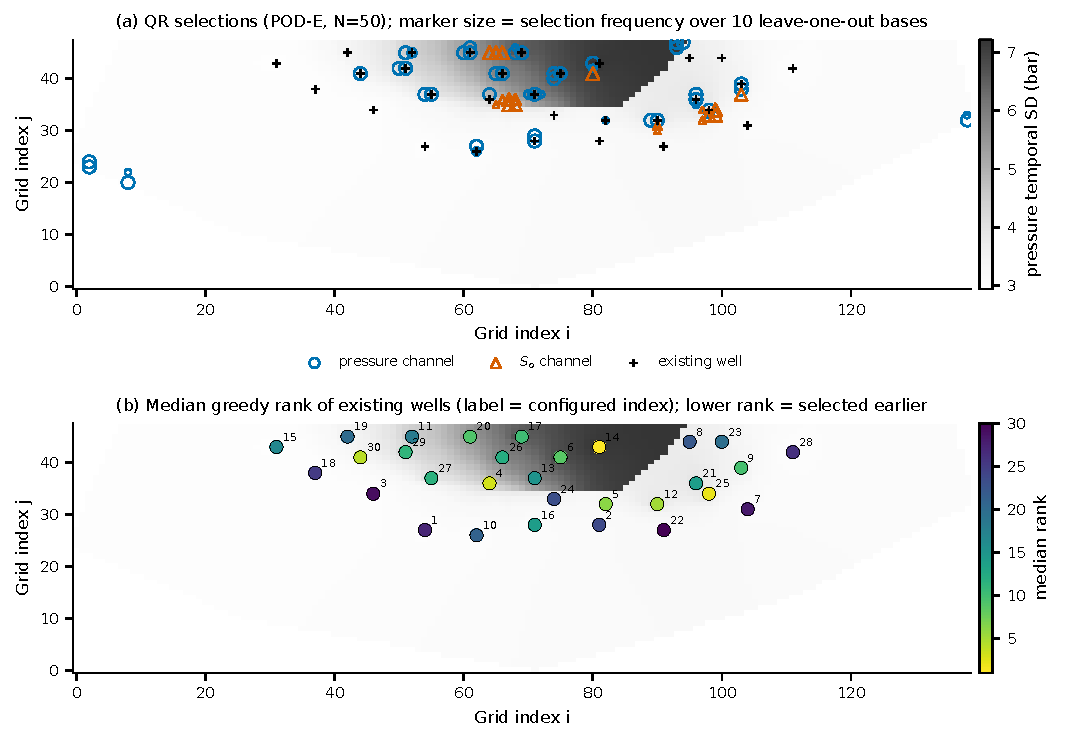
\includegraphics[width=\textwidth]{../../../../studies/brugge_sparse_sensing/figures/fig7_sensor_maps.pdf}
\caption{Location of selected sensors in P2. (a) QR selections on POD-E for $N=50$ channels; marker size is the fraction of the ten leave-one-out bases in which a channel was selected (circles: pressure; triangles: $S_o$); background: temporal standard deviation of pressure averaged over all ten scenarios (descriptive background only); crosses: existing wells. (b) Median DG rank of each existing well over the ten folds (colour; rank 1 is selected first), labelled by configured order.}
\label{fig:maps}
\end{figure}

\begin{table}[tbp]
\centering
\small
\caption{Single-thread wall time (median of repeated runs) for P2 fold 1; online times are per snapshot, amortised over the 133 held-out snapshots of the fold solved jointly ($M=9{,}900$ channels, 1{,}197 training snapshots, $r=16$). Hardware: MacBook Pro, Apple M2 Pro, 12 (8 performance, 4 efficiency) cores, 16 GB memory; Python 3.12.12, NumPy 2.5.2.}
\label{tab:cost}
\begin{tabular}{@{}llr@{}}
\toprule
Step & Stage & Time \\
\midrule
POD basis (thin SVD) & offline & 1.18 s \\
TBMD basis (Tucker/HOOI, ranks (48,48,2,16)) & offline & 8.9 s \\
QR placement, $N=r$ & offline & 2.1 ms \\
QR + DG placement, $N=300$ & offline & 1.00 s \\
DG ranking of 30 wells & offline & 3.2 ms \\
LS estimate, 30 wells & online, per snapshot & 0.8 \si{\micro\second} \\
$\ell_1$ (ADMM) estimate, 30 wells & online, per snapshot & 32 \si{\micro\second} \\
LS estimate, 30 grid channels & online, per snapshot & 0.7 \si{\micro\second} \\
$\ell_1$ (ADMM) estimate, 30 grid channels & online, per snapshot & 23 \si{\micro\second} \\
\bottomrule
\end{tabular}
\end{table}

